% !TeX encoding = utf8
% !TeX spellcheck = fr

\chapter{Espace aérien, trafic et vol en équipe}\label{cha:airspace}

\begin{framed}
	\begin{center}
		\xc{} est entièrement développé par des bénévoles.\\
		Cette documentation aussi.\\
		Si vous y voyez des imperfections, vous pouvez facilement les faire disparaître~:\\
		\xcsoarwebsite{/develop/}
	\end{center}
\end{framed}

Les données spécifiques à l'utilisation de l'espace aérien peuvent être chargées dans \xc.
Elles sont utilisées pour l'affichage des différents types d'espaces et pour la détection de l'entrée/sortie de l'aéronef de ces espaces.

Deux fichiers d'espaces aériens peuvent être paramétrés. Le premier est la base de donnée principale de l'espace aérien.
Le second est dédié aux espaces changeants fréquemment (valables sur une courte période) comme les espaces définis dans des NOTAM.

Il est de la responsabilité de l'utilisateur de s'assurer que les données relatives aux espaces aériens sont à jour.

À l'aide d'un FLARM connecté, le calculateur affiche aussi des informations sur les autres aéronefs environnants équipés de FLARM et sur les obstacles dangereux.

Une fonctionnalité ``Code équipe'' permet à des équipes de pilotes d'échanger leurs positions par radio en utilisant un code qui ne peut signifier quelque chose que pour leurs coéquipiers. Ces données sont encodées et décodées par le calculateur.


\section{Affichage des espaces aériens}

Les espaces aériens à usage spécial sont représentés sur la carte par une zone ombrée avec une bordure épaisse.
La couleur et le motif sont spécifiques au type d'espace et peuvent être configurés par l'utilisateur.
En fonction du paramétrage, il est possible d'afficher tous les espaces, seulement ceux sous une certaine altitude, seulement ceux compris entre deux altitudes, ou bien seulement ceux qui sont sous le planeur.  
\sketch{figures/airspace.png}

Les modèles de représentation peuvent être opaques, transparents au milieu, hachurés  continus ou pointillés. Les modèles non-opaques sont partiellement transparents en ce qui concerne le relief et la topographie, mais \emph{ne sont pas} transparents pour les espaces aériens se chevauchant. Cependant, quand des espaces se chevauchent, leurs bordures sont affichées. C'est-à-dire que pour les modèles d'espace aérien qui ne sont pas mutuellement transparents, toutes les frontières d'espace aérien sont dessinées au-dessus des zones d'espace aérien.

L'affichage et l'alerte de pénétration d'une classe d'espace aérien peuvent être activé ou désactivé individuellement par l'utilisateur. Voir la section~\ref{sec:airspace-filter}.

Les couleurs par défaut des espaces de classes C, D, E et F sont conformes aux cartes OACI.


\subsection*{Événements d'intrusion}

Trois types d'événements sont détectés par \xc{} concernant les espaces aériens~:
\begin{description}
\item[Incursion prédite] Cet évènement est activé quand la trajectoire du planeur est estimée entrer dans l'espace aérien dans un laps de temps donné. Ce laps de temps est le ``Temps d'alerte'' du menu de configuration.

Les calculs utilisent la moyenne de la direction de la trajectoire sur une longue durée~: ceci permet de prédire l'incursion dans une zone même quand le planeur dérive, du fait du vent, en spirale.


%{\it DIAGRAM SHOWING DETECTION OF PREDICTED INCUSION WHEN CIRCLING AND
%  CRUISING}

\item[Entrée] Évènement activé lors de l'entrée dans un espace aérien.
\item[Sortie] Évènement activé lors de la sortie d'un espace aérien.
\end{description}
En toutes circonstances, le pourtour de l'espace est défini par les altitudes minimale et maximale ou par les niveaux de vol, tels que définis dans le fichier des espaces aériens.

Les alertes d'incursion dans un espace aérien sont produites même si le lieu de pénétration dans la zone est en dehors de l'écran.

Quand une altitude barométrique est disponible, celle-ci est utilisée à la place de l'altitude fournie par le GPS pour détecter l'intrusion dans les espaces aériens. Ceci rend le système conforme aux conventions usuelles de calcul de violation des espaces aériens, basé sur le QNH.


\section{Alertes et espaces aériens}

Les alertes d'espaces aériens sont progressives~:
\begin{description}
\item[Aucune] L'aéronef est à l'extérieur et à une certaine distance de tout espace aérien.
\item[\colorbox{AirspaceYellow}{Near}] L'aéronef se rapproche et va bientôt entrer dans un espace aérien.
\item[\colorbox{AirspaceRed}{Inside}] L'aéronef est à l'intérieur d'un espace aérien.
\end{description}

En permanence, \xc{} contrôle la position de l'aéronef par rapport à tous les espaces aériens du fichier d'espaces aériens et gère les niveaux d'alertes pour chaque espace. Les alertes sont filtrées en accord avec les préférences définies par l'utilisateur~: ainsi certains types d'espaces peuvent être totalement ignorés.
\sketch{figures/airspacewarning.png}
La séquence des évènements signalés en entrant dans une zone est constituée de deux alertes~: niveau~1 = proche = ``near'' et niveau~2 = à l'intérieur = ``inside''.

À chaque accroissement du niveau d'alerte (supérieur à~0), et quelque soit l'espace, la boîte de dialogue s'affiche avec un bip sonore. Quand il n'y a plus d'espace ayant un niveau d'alerte au-dessus de~0, la boîte de dialogue se ferme automatiquement.

\subsection*{La boîte de dialogue Alerte Espace Aérien}

La boîte de dialogue ``Alerte Espace Aérien'' peut comporter jusqu'à quatre alertes individuelles. Le fond des éléments de la liste est rouge pour signifier que l'aéronef est dans la zone, jaune s'il en est proche. Une alerte qui a été reconnue est écrite en gris.

Chaque alerte occupe deux lignes et comporte les détails suivants~:\\
\verb+<NOM et Classe>   <NIVEAU SUP.>  <Niveau Alerte>+  \\
\verb+<Temps et distance si à l'extérieur> <NIVEAU INF.>+

Les alertes de la liste sont mises à jour continuellement.
Voici un exemple~:\\
\verb+ECRINS 1000m/sol No (1000 m    AGL  +\colorbox{AirspaceYellow}{near}\\
\verb+30 sec dist 2130 m             GND+

Ce qui signifie que l'aéronef est à 30~secondes environ et 2130~m horizontalement de la bordure de la zone des ECRINS. Survol interdit en dessous de 1000~m sol.

Un autre exemple~:\\
\verb+R196A1 Est GAP (Notam         FL195  + \colorbox{AirspaceRed}{inside}\\
\verb+                     1006 m   AGL+

Ce qui signifie que l'aéronef est dans la zone R196A1 de plafond FL~195 et de base 1006~m sol. Cette zone est spécifiée par NOTAM (zone de parachutage au-dessus de Gap).

À chaque alerte d'espace aérien, la boîte de dialogue s'ouvre et vous pouvez accéder aux détails de la zone en question en appuyant dessus.
\begin{center}
\includegraphics[angle=0,width=\linewidth,keepaspectratio='true']{figures/alerteespaceaerien2.png}
\end{center}


\subsection*{Accusé de réception des alertes}

Quand la boîte de dialogue des alertes est ouverte et qu'une alerte est active, la boîte de dialogue peut être fermée sans accuser réception des alertes en appuyant sur \bmenug{Fermer} ou sur Échap. (sur PC).

Quand une ou plusieurs alertes sont visibles dans la boîte de dialogue des alertes, une alerte peut être acquiescée en appuyant sur l'un des boutons au bas de la boîte de dialogue. 

Signification des boutons d'asquiescement des alertes~:
\begin{description}
\item[OK Alert.] Accuse réception du niveau de l'alerte courant. Une nouvelle alerte apparaîtra seulement si le niveau d'alerte augmente.
\item[OK Esp.] Accuse réception de tous les niveaux d'alerte présents et futurs concernant cet espace aérien, et ceci tant que le planeur est éloigné de moins de 2,5~km horizontalement et 500~m verticalement.
\item[OK Jour] Accuse réception de tous les niveaux d'alerte présents et futurs concernant cet espace aérien pour le reste du vol (ou jusqu'au redémarrage d'\xc.
\item[Activer] Invalide l'accusé de réception d'un espace aérien et ré-active les alertes de cet espace.
\item[Fermer] Ferme la boîte de dialogue des alertes, sans accuser réception des alertes affichées. La boîte de dialogue s'ouvre à nouveau automatiquement si le niveau d'alerte augmente.
\end{description}

Remarque~: les différents boutons ne sont pas tous visibles pour tous les niveaux d'alerte. En particulier, si à l'intérieur d'un espace aérien, le bouton \bmenug{OK Alert.} n'apparaît pas, cela signifie que l'espace concerné n'est plus une menace imminente mais qu'en fait vous êtes déjà dedans.

Règles générales d'utilisation de la boîte de dialogue des alertes~:
\begin{itemize}
\item Ne pas accuser réception d'une alerte qui concerne un espace que vous devez ou comptez contourner.
\item Le bip de l'alerte est seulement émis lors de l'accroissement du niveau de l'alerte.
\item Le système d'alerte est conçu pour permettre de spiraler près d'un espace aérien sans stresser inutilement le pilote en générant des alarmes en trop.
\end{itemize}

Quand on accuse réception d'une alerte d'espace aérien avec \bmenug{OK Esp.}, il n'est plus représenté que par son pourtour, les hachures sont supprimées.

Quand il va y avoir pénétration dans un espace aérien ou qu'il y a déjà pénétration, une alarme sonore est émise avec un message détaillé décrivant le type d'espace (dont la classe, le plancher et le plafond en altitude ou en niveau de vol).

Les alertes ayant été acquiescées sont répétées après un certain temps qui est configurable dans le menu Option Système sous le nom de ``Durée d'acquiescement''.

L'acquiescement d'une alerte ne s'applique qu'à un espace aérien donné. Si un planeur entre dans l'espace~A et que le pilote accuse réception de cette alerte et qu'en même temps il s'approche aussi d'un espace~B, une alerte sera signalée concernant l'espace~B.

\tip Si vous souhaitez que les alertes acquiescées ne soient pas répétées, il est conseillé de mettre une grande valeur au paramètre ``Durée d'acquiescement''.

Les alertes concernant un espace sont effacées automatiquement de la boîte de dialogue quand la position du planeur ainsi que sa trajectoire future estimée sont en dehors de l'espace considéré.

Plusieurs alertes peuvent se déclencher simultanément si l'aéronef (ou sa trajectoire estimée) pénètre dans plusieurs espaces.


\section{Recherche et détails des espaces}\label{sec:airspacedetails}

Pour les terminaux tactiles ou ayant une souris, quand un espace aérien est visible sur la carte, il suffit de le toucher ou de cliquer dessus pour obtenir les détails le concernant. La liste des éléments de la carte apparaît et donne un aperçu des points de virages, terrains, position actuelle et espaces aériens qui sont à l'endroit sélectionné. Les espaces aériens sont affichés de la même façon que lors des alertes. La recherche donne tous les espaces aériens visibles sur la carte qui se chevauchent à l'endroit sélectionné.
\sketch{figures/airspace_mapelements.png}
Le fait de sélectionner un espace aérien dans la liste et d'appuyer sur \button{Détails} ou sur entrée permet de voir tous les détails concernant l'espace choisi.

\tip Une autre façon de rechercher les espaces aériens et autres informations~: en mode PAN~ON (panoramique), déplacer la carte pour positionner le curseur à l'endroit désiré.  Appuyer sur le bouton  \button{Qu'y a-t-il ici~?} pour afficher la même liste des éléments de la carte à cet endroit.



\subsection*{Fenêtre de recherche et filtrage des espaces aériens}\label{sec:airspace-filter}

La boîte de dialogue de filtrage des espaces aériens permet d'activer ou de désactiver les alertes et l'affichage pour chaque classe d'espace.

On y accède de plusieurs manières~:
\begin{itemize}
\item Depuis le menu principal \bmenug{Info. 3}\blink\bmenug{Espaces Aériens}.
\item Depuis le menu Espace aérien dans Config. -- Système -- Carte, puis en appuyant sur le bouton \button{Filtre}.
\end{itemize}

\sketch{figures/airspacefilter.png}
Pour utiliser cette boîte de dialogue, déplacer la liste vers le haut ou vers le bas. La touche Entrée alterne entre les différentes alertes et les options d'affichage.

\subsection*{Gestion des espaces aériens}

En appuyant sur \button{Parcourir}
la boîte de dialogue de gestion des espaces aériens s'affiche. Son utilisation est similaire à celle de la boîte de dialogue de gestion des points de virage. Il est possible de rechercher sur les critères de nom, de distance, de cap et de type (classe).
\sketch{figures/airspacelookup.png}

Quand l'espace aérien est trouvé, il est possible de le désactiver pour la journée ou de le ré-activer s'il ne l'était plus.


\section{Analyses}

L'une des pages de la boîte de dialogue ``Analyses'' montre une coupe verticale de l'espace aérien. On y accède par~:
\menulabel{\bmenug{Info. 1}\blink\bmenug{Analyses}}

Cette section montre les 50~km de l'espace aérien dans la direction du planeur (axe des X) et son altitude (axe des Y). L'altitude du planeur est indiquée par un flèche blanche sur la gauche. Cette page est très utile pour visualiser l'imbrication des espaces aériens, qui peut être complexe dans certaines situations.

\begin{center}
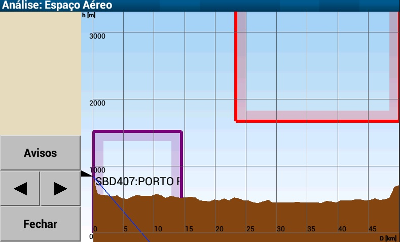
\includegraphics[angle=0,width=0.8\linewidth,keepaspectratio='true']{figures/analysis-airspace.png}
\end{center}

Le bouton ``Avertissements''
ouvre directement la fenêtre des alertes quand le planeur est à proximité ou à l'intérieur d'un espace aérien.
\begin{center}
\includegraphics[angle=0,width=0.8\linewidth,keepaspectratio='true']{figures/analysis-airspace2.png}
\end{center}


\section{Trafic et FLARM}

Si \xc{} est connecté à un FLARM, les aéronefs équipés d'un FLARM sont visibles sur la carte. Chaque aéronef reçu est représenté par un cercle rouge en pointillés.

\warning Il ne faut pas utiliser \xc{} en tant qu'anti-collision. Les dispositifs FLARM et leur alertes sonores sont bien plus efficace pour aider le pilote à avoir conscience du trafic. Et cela ne doit pas empêcher de regarder dehors~!

Remarque~: à moins de spiraler, le niveau de zoom habituel ne permet pas de distinguer aisément les autres FLARMs du secteur. En spirale le niveau de zoom peut être correct, mais le changement constant de cap et la latence du PDA font que l'aide à la localisation des autres aéronefs n'est ni très efficace ni fiable.


\subsection*{Affichage du trafic sur la carte}

Les trafics FLARM sont représentées sur la carte par des flèches rouges dont la pointe montre la direction de l'aéronef ayant un FLARM ainsi que le risque\config{flarm-on-map} de collision. Notez que l'orientation des flèches dépend du mode d'affichage de la carte. Par exemple, si le mode d'affichage est ``Route en haut'', les flèches pointent vers la direction relative des trafics par rapport au planeur. Si le mode d'affichage est ``Nord en haut'', les flèches pointent vers la direction des routes absolues des trafics.
\sketch{figures/flarmmap.png}

L'affichage sur la carte des données d'identification des FLARMs (numéro de concours, nom du pilote, immatriculation) est possible par l'intermédiaire d'un fichier OACI d'identification de trafic aérien pour FLARM. Voir section~\ref{sec:flarm-ident-file} pour plus de détails sur le format du fichier. Les aéronefs ayant activés l'option ``anonyme'' de leur FLARM ne seront identifiés que par une flèche, aucune donnée d'identification ne sera affichée.


\subsection*{Radar FLARM}

Pour palier à cette situation, quand un trafic FLARM est reçu, \xc{} affiche une petite fenêtre de type FLARM du point de vue de l'aéronef. Le trafic FLARM est représenté de la même façon, mais les trafics menaçants sont rendues plus visibles en étant entourées de un ou deux cercles rouges. Le coin d'affichage de cette vue radar FLARM peut être paramétré\config{flarmradar-place}.

Cette vue de radar FLARM est affichée en mode ``Route en haut'' et un petit planeur, au centre, rappelle ce mode d'affichage. L'échelle est linéaire jusqu'à 2000~mètres. En fond d'écran il y a 2~cercles~: le premier a un rayon de 1000~m et le second de 2000~m. Le trafic distant de plus de 2~km du centre est représenté sur le cercle des 2~km.
\sketch{figures/flarmrose.png}

Tous les affichages du trafic FLARM montrent le trafic avec les mêmes couleurs, symbolisant la menace potentielle ou le vol en équipe. Les couleurs sont~:
\begin{itemize}
\definecolor{warning}{rgb}{1,0.64,0}
\definecolor{teammate}{rgb}{0.45,1,0}
\item \textcolor{black} {Noir pour le niveau~0, pas de danger.} 
\item \textcolor{warning} {Jaune pour le niveau~1, attention.}
\item \textcolor{red} {Rouge pour les niveaux~2 et~3, alerte.}
\item \textcolor{teammate} {Vert pour un membre de l'équipe.}
\item \textcolor{blue} {Bleu pour le trafic sélectionné.}
\end{itemize}

Pour tout trafic dont la menace est supérieure à~1, la différence d'altitude arrondie est affichée. L'affichage montre la différence d'altitude arrondie à~100. Un petit triangle noir (au-dessus du~1 sur la figure) indique si le trafic est au-dessus ou au-dessous de vous. L'exemple ci-dessous montre un trafic environ 100~m au-dessus (pour une altitude en mètres) car il pointe vers le haut. 

Si activé, l'affichage de type radar FLARM peut être supprimé en appuyant sur ``Fermer'' ou ``Entrer'' suivant les plateformes.
La même action permet de ré-afficher le radar. Quand un nouveau trafic apparaît, ou si le radar émet une alerte de collision, le ré-affichage est automatique.

\subsection*{Fenêtre de dialogue du trafic FLARM}\label{sec:flarm-traffic}

Dés que le FLARM détecte un trafic et que la petite vue du radar apparaît\config{flarmdisplay} vous pouvez appuyer dessus pour la mettre en plein écran.
L'affichage plein écran offre toutes les informations
\menulabel{\bmenug{Info. 1}\blink\bmenut{FLARM}{Radar}}
concernant les trafics détectés par la FLARM. Suivant le paramétrage, il disparaît automatiquement quand il n'y a plus de trafic aux alentours.

\begin{center}
\includegraphics[angle=0,width=0.8\linewidth,keepaspectratio='true']{figures/dialog-flarm1.png}
\end{center}

Seuls quelques boutons de contrôle sont présents. De haut en bas~:
\begin{description}
\item[Nord en haut] Si coché, l'affichage est en mode ``Nord en haut''. Sinon c'est ``Route en haut''.
\item[A. Zoom] \gesture{Haut - Bas} Réglage automatique du zoom pour que les trafics soient parfaitement visibles. Si pas coché, le zoom doit être ajusté manuellement. Le geste Haut - Bas active le zoom automatique.
\item[Avg/Alt] \gesture{Droite - Gauche} Bascule de l'affichage entre vario moyen et altitude moyenne à côté du trafic.
\item[Détails] \gesture{Bas - Droit} À l'aide du bouton, une boîte de dialogue concernant le trafic choisi apparaît, montrant tous les détails.
\item[+/-] \gesture{Haut/Bas} Change manuellement le zoom de 500~m à 1000~m. Les commandes de zoom par geste sont toujours possibles.
\item[$\triangleleft$/$\triangleright$] \gesture{Gauche/Droite} Passage d'un trafic à l'autre.
\end{description}

\begin{center}
\begin{tabular}{c c}
\includegraphics[angle=0,width=0.5\linewidth,keepaspectratio='true']{figures/cut-flarm2.png}&
\includegraphics[angle=0,width=0.5\linewidth,keepaspectratio='true']{figures/cut-flarm3.png}\\
\end{tabular}
\end{center}
Les trois copies d'écran, prises en séquence, montrent le passage à proximité de 2~planeurs équipés de FLARM. Les informations détaillées sont en couleur et suivent le code de couleur décrit plus haut.
Dans les 4~coins de l'écran radar les informations concernent le trafic sélectionné (si plusieurs trafics dans le secteur)~:
\begin{description}
\item[Haut gauche] Si disponible, identifiant FLARM du trafic sélectionné.
\item[Haut droite] Vario du trafic, à partir des altitudes successivement reçues.
\item[Bas gauche] Distance au trafic.
\item[Bas droite] Différence de hauteur entre l'aéronef et le trafic. 
\end{description}

Entre la première et la seconde copie d'écran, 15~secondes sont passées. Le trafic bleu sélectionné montait à 3,4~m/s et ne constituait pas une menace de collision envers le planeur. Pendant ce temps, le `DC' a viré plus sur la gauche, devenant une menace et passant alors en rouge. Le zoom du radar FLARM est alors passé de 1000~m à 500~m. La dernière copie d'écran montre que le `DC' est en montée continue, le niveau de `menace' est repassé à~1, son affichage est devenu jaune, il ne semble plus être une menace.


\section{Vol en équipe}\label{sec:team-flying}

Le code équipe est un moyen, donné aux pilotes d'une équipe, de communiquer entre eux leur position de façon concise et avec précision. Le principe est que chaque pilote calcule un code à 5~caractères à l'aide du calculateur décrivant sa position par rapport à un point de virage commun à toute l'équipe. Les pilotes s'échangent leur codes par radio, et en entrant ces codes, ils peuvent visualiser avec précision leurs équipiers sur la carte.

Pour générer un code équipe, tous les pilotes doivent choisir un point de virage commun, qui est leur référence. Ceci se fait avec la fenêtre de dialogue ``Code équipe''.
\menulabel{\bmenug{Info 2}\blink\bmenut{Team}{Code}}
Le point de virage de référence est défini à l'aide du bouton \button{Définir WP}.
Le point de virage sélectionné dans la liste sera le point de virage de référence, et devra être le même pour tous.

En vol, le pilote peut donner son code équipe, personnel, à son équipier, à l'aide de la fenêtre ``code équipe'', afin que celui-ci dispose de votre position de façon cryptée. Quand il entend le code d'un équipier, il appuie sur \button{Définir code} pour ouvrir le fenêtre de saisie de texte permettant d'entrer le code de son équipier.
\sketch{figures/dialog-teamcode.png}


Après avoir entré le code de son équipier, la distance entre les 2~planeurs est affichée ainsi que le cap à suivre pour rejoindre l'équipier. Ces valeurs sont mises à jour dans la fenêtre.

\subsection*{Recherche d'un code FLARM}
\xc{} supporte aussi les codes d'équipe cryptés du projet FlarmNet. Le bouton \button{Capture Flarm}
permet d'accéder à la base de données FlarmNet ainsi qu'aux données FLARM de \xc{} pour trouver un équipier. La simple recherche d'un numéro de concours affiche potentiellement le code FLARM désiré. En sélectionnant l'entrée voulue dans la base de données à partir des éléments listés, vous pouvez localiser votre équipier à distance. Voir la section~\ref{sec:flarm-ident-file} pour plus de détails.

\menulabel{\bmenug{Info. 2}\blink\bmenut{Liste du}{trafic}}
Des fonctions similaires donne accès à la fenêtre de dialoque des détails du FLARM. Cela vous laisse aussi chercher un numéro de concours dans la base de données et vous donne des détails sur ce dernier. 

\begin{center}
\includegraphics[angle=0,width=0.8\linewidth,keepaspectratio='true']{figures/dialog-flarmdetails.png}
\end{center}

Même si \xc{} ne gère qu'un seul équipier avec un point de virage prédéfini, il n'est pas limité en nombre de ``copains'' dont vous connaissez l'identifiant FLARM. Il est très probable que vos amis ne soient enregistrés dans aucune base de données. Mais si vous vous rapprochez de vos amis en vol, affichés les détails à partir de l'écran radar FLARM, associez lui une couleur, et \xc{} identifiera la réponse de ce FLARM à votre ami dans le futur.
